\section{図・表の挿入}
\subsection{図}
テストを図\ref{fig:test}に示す.
\begin{figure}[htb]
% h:here, t:top, b:bottom, p:page
  \begin{center}
    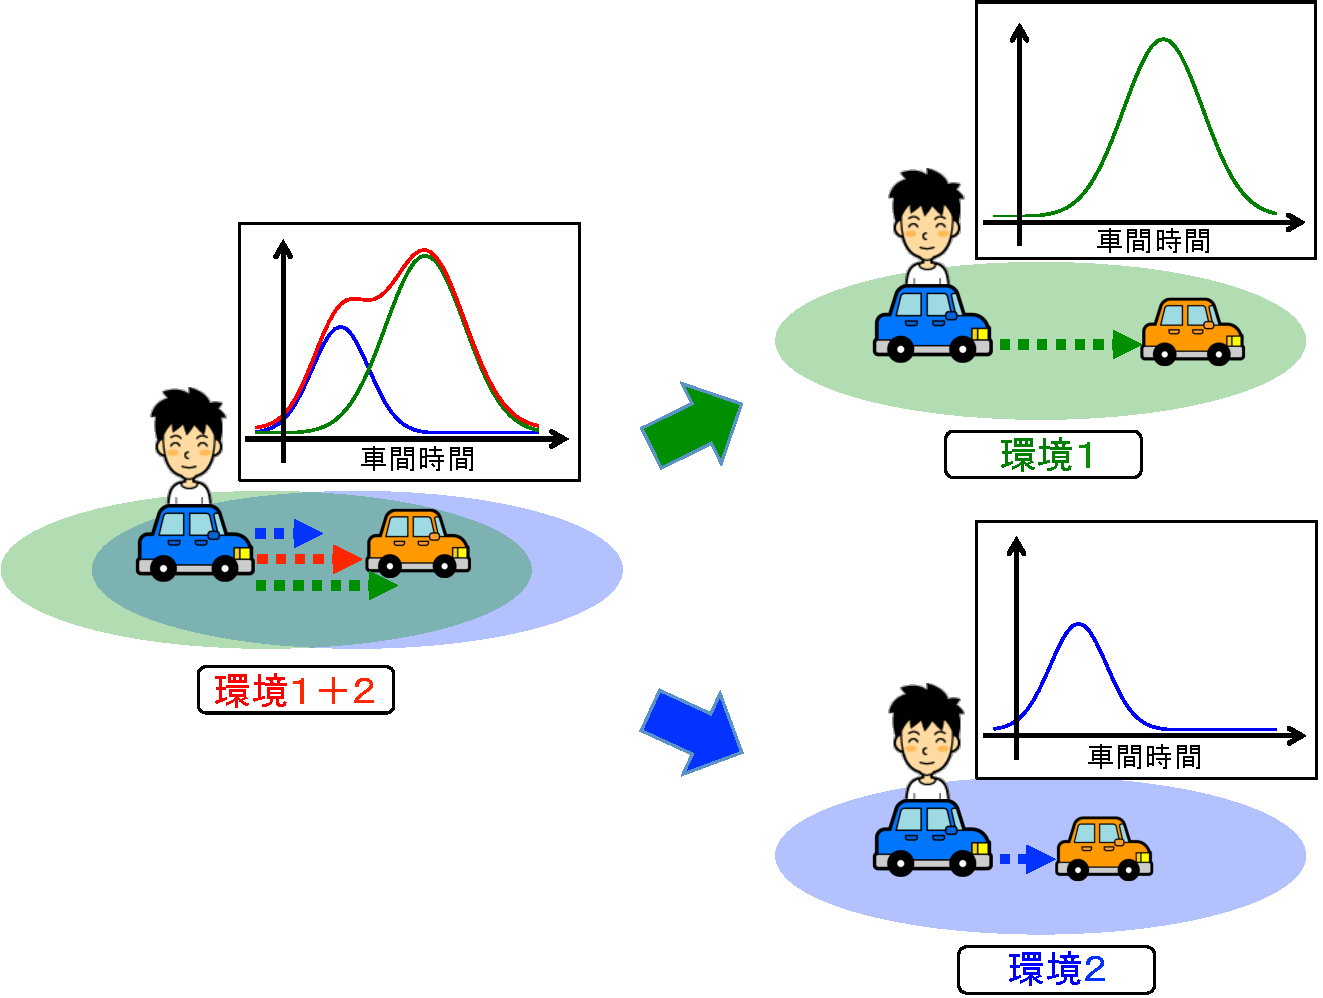
\includegraphics[width=7.0cm]{./images/test.pdf}
    \caption{テストの図}
    \label{fig:test}
  \end{center}
\end{figure}

\subsection{表}
表\ref{tab:price}は\url{http://www.latex-cmd.com/fig_tab/table01.html}から持ってきたものである.
\begin{table}[htb]
  \begin{center}
    \caption{値段表}
    \begin{tabular}{|l|c|r||r|} \hline
      メニュー & サイズ & 値段 & カロリー \\ \hline \hline
      牛丼 & 並盛 & 500円 & 600 kcal \\
      牛丼 & 大盛 & 1,000円 & 800 kcal \\
      牛丼 & 特盛 & 1,500円 & 1,000 kcal \\ \hline
    \end{tabular}
    \label{tab:price}
  \end{center}
\end{table}
% excelで言うセルの結合をしたかったら\mulricolumnとか\clineとかを使うらしい.
